\chapter{Training data of CFD results to train surrogate model}
In our case, 80 DOEs are generated and steady state 3D CFD analysis has been performed for these 80 shapes. The solver parameters used are as follows:
\begin{table}[H]
	\caption{Flow conditions and solver parametres for all DOE shapes}
	\label{Flow conditions and solver parametres for all DOE shapes}
	\centering
	\begin{tabular}{ll}
		\hline \hline
		Parameters & Value \\ 
		\hline \hline
		Reynolds number based on volume Re & $ 3.01 \ast 10^6 $ \\
		Pressure, N/m2 & 87500 \\
		Density, Kg/m3 & 1.057 \\
		Speed, m/s & 51 \\
		Mesh & Hexahedral mesh using blockMesh and snappyHexMesh \\
		Solver & SimpleFOAM (Incompressible steady state solver) \\
		Turbulent..? & Yes \\
		Turbulence model & K-Omega SST \\
		\hline \hline
	\end{tabular}
\end{table}
\section{Grid Convergence study}

Effect of grid size on the overall results by  changing the number of cells in self similar mesh has been carried out. Below is the plot of variation of pressure and viscous drag with number of cells for a simulation. As mentioned by \cite{Suman2011} , when the percentage change in the values is less than 5 \%, then the solution is reported to have grid convergence.

\begin{table}[H]
	\caption{Grid convergence study}
	\label{Grid convergence table}
	\centering
	\begin{tabular}{ccc}
		\hline \hline
		Cells & Pressure Drag (N) & Viscous Drag (N) \\
		\hline \hline
		376380 & 1.1  & 11.02 \\
		604375  & 2.2  & 11.68 \\
		840565  & 2.02  & 12.1 \\
		994864  & 2.09  & 12.24 \\
		1563471  & 2.12 & 12.5 \\
		\hline \hline
	\end{tabular}
\end{table}

\begin{figure}[H]
	\centering
	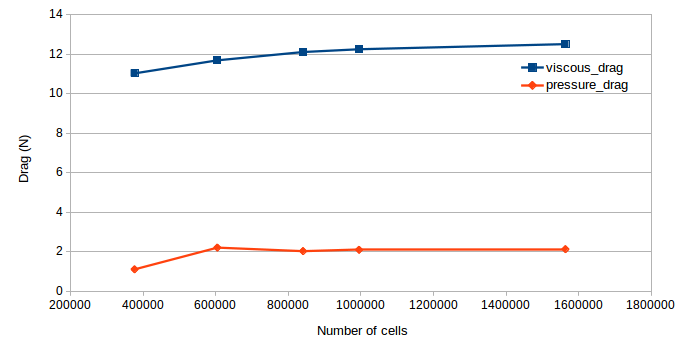
\includegraphics[width=300 pt]{surrogate_model_CFD_results/Grid_convergence.png}
	\caption{Variation of pressure and viscous drag with number of cells}
	\label{Grid convergence plot} %      only if needed
\end{figure}
Since there is no considerable amount of change in drag values, the number of cells are taken are around 1 million instead of 1.5 million for all the cases. This saves computational time.

\section{Results of CFD simulations}
\begin{figure}[H]
	\centering
	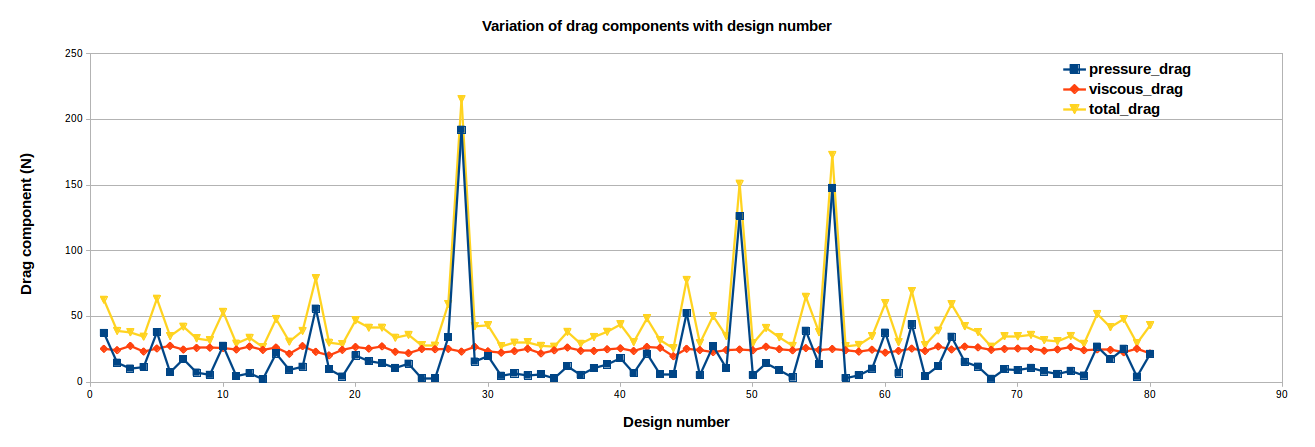
\includegraphics[width=450 pt]{surrogate_model_CFD_results/Drag_components.png}
	\caption{Variation of pressure and viscous drag with design number}
	\label{Drag components plot} %      only if needed
\end{figure}

\begin{figure}[H]
	\centering
	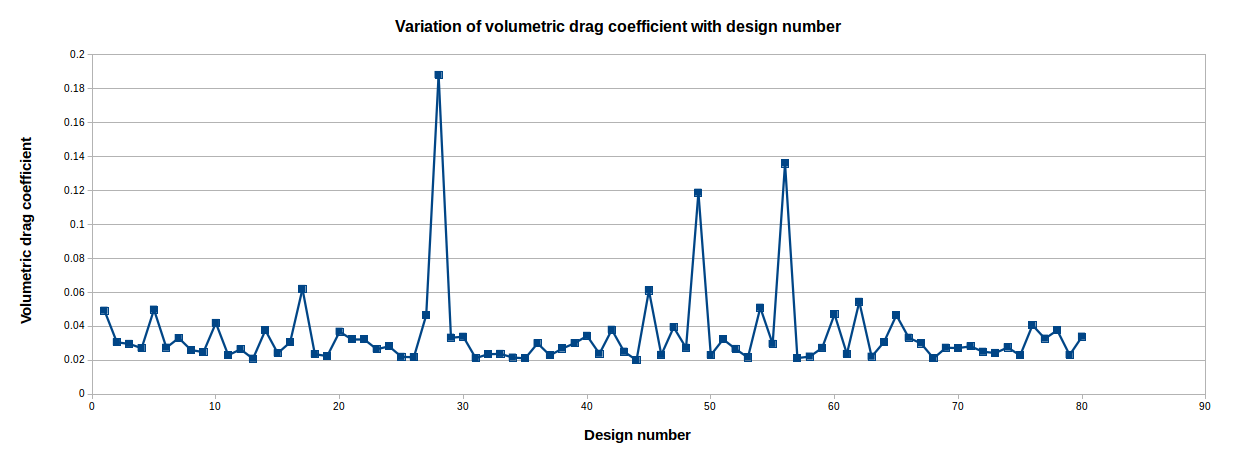
\includegraphics[width=450 pt]{surrogate_model_CFD_results/Volumetric_drag_coeff.png}
	\caption{Variation of volumetric drag coefficient with design number}
	\label{Volumetric drag coefficient plot} %      only if needed
\end{figure}

\section{Testing the accuracy of surrogate model}

Three surrogate models mentioned in \ref{Three surrogate models} has been fit to the above data. Then ten random design points has been generated in the domain for testing purpose. The results are shown in the following table \ref{Accuracy of different surrogate models}.

\begin{table}[H]
	\caption{Accuracy of different surrogate models}
	\label{Accuracy of different surrogate models}
	\centering
	\begin{tabular}{cccc}
		\hline \hline
		Random Exp.No	&Kriging (\% Error)	&PRS (\% Error)	&RBF (\% Error) \\
		\hline \hline
		1	&7.36	&2.70	&9.79 \\
		2	&2.74	&9.48	&26.03 \\
		3	&4.13	&10.48	&65.21 \\ 
		4	&0.49	&5.81	&11.42 \\
		5	&0.28	&8.79	&23.59 \\
		\hline \hline
		Avg. \% Error	&3.00	&7.45	&27.21 \\
		\hline \hline
	\end{tabular}
\end{table}
From the above results we can observe that Kriging predicted the functional behaviour with more accuracy. Radial basis function is having more error because the amount of training data is not sufficient in our case. Accuracy of polynomial response surface is between Kriging and Radial basis function. So, Kriging has been selected for coupling with optimiser in our study.
